\documentclass[12pt,lettersize,journal,onecolumn]{IEEEtran}
\usepackage{amsmath,amssymb,graphicx,booktabs,setspace,etoolbox}
\doublespacing
\AtBeginEnvironment{table}{\singlespacing}
\AtBeginEnvironment{figure}{\singlespacing}
\begin{document}
\title{Supplementary Materials for\\Ask Before You Transmit:
An Energy-Frugal Evidence-Level Semantic Communication System for UAV
Visual Question Answering}
\author{Qiankun Zhang, Yue Liu, Zhijin Qin, Hongbin Liang, and Nelson L. S. da Fonseca}
\maketitle

\section{Evaluation Scope and Provenance}
The reported comparisons use existing paired branch outcomes with
image-disjoint training, validation, and test partitions. Count
calibration is fitted on training images only. Sender features
are checked against original detector records, rather than inferred
from the names of fields in a prediction log.
The main channel sweep uses fixed branches, the type rule, and
training LUTs on all three VisDrone channels. These policies do
not use per-query sender-count inputs.

For reproducibility, we distinguish usable records from archived
diagnostics. Historical learned-router runs that used answer-derived
polarity or annotation-derived viewpoint/risk inputs are not used
as performance evidence. A later audit also found that some extra-task
records stored received counts in a field named raw detector count.
This changes $279$ actual feature vectors on Rayleigh and $33$ on
Rician, including training, validation, and test. Those full-model
and affected ablation records are excluded from the reported
learned-policy comparisons. AWGN has no such input differences.
The fixed-policy outcomes and their receiver counting labels are
unaffected by this sender-feature issue.

The DroneVehicle target-data fit and matched-receiver evaluation
restore sender counts from the original detection boxes.
DroneVehicle corrects $18$ raw-field records. For the matched
receivers, each corrects $44$ raw-field records, of which $33$
change the scaled/clipped feature vector. The interrupted first
receiver run is archived, not combined with the corrected run.
All original logs remain unchanged. No result in this paper
establishes frozen VisDrone-router transfer to DroneVehicle.

\section{Verified AWGN Learned-Policy Comparison}
Table~\ref{tab:awgn} retains the full AWGN comparison, including
cases in which a simpler method matches or exceeds the MLP.
Each learned point uses the same $104$ test images and $5{,}616$
question/SNR decisions. The validation selection procedure and
the $26$ prices are those defined in the main paper.

\begin{table}[t]\centering
\caption{AWGN accuracy (\%) and accounted system energy (J/query).
MLP-based configurations use ten-seed means; accuracy uncertainty
is one sample standard deviation. The two operating-point columns
do not impose the same absolute accuracy target on each method.}
\label{tab:awgn}\footnotesize
\begin{tabular}{@{}lrrrr@{}}\toprule
 & \multicolumn{2}{c}{No energy price} & \multicolumn{2}{c}{Validation-selected}\\
Configuration & Accuracy & Energy & Accuracy & Energy\\\midrule
Linear & 68.02 & 11.86 & 67.08 & 3.17\\
Full MLP & $67.92\pm0.19$ & 13.38 & $67.89\pm0.35$ & 3.71\\
No detector inputs & $67.96\pm0.04$ & 8.88 & $66.90\pm0.33$ & 3.60\\
No SNR input & $67.86\pm0.24$ & 13.65 & $67.96\pm0.16$ & 3.76\\
Question type only & $67.47\pm0.00$ & 14.65 & $67.47\pm0.00$ & 14.65\\
\bottomrule\end{tabular}
\end{table}

The unpriced full MLP is slightly less accurate and more costly
than the linear reference. Removing detector inputs causes little
unpriced accuracy change, but its validation-selected point has
lower test accuracy than the full MLP point. Removing SNR produces
only a small unpriced difference and does not reduce accuracy
at the selected point. These observations do not establish a
general benefit or lack of benefit for CSI. They apply to the
specified inputs and channel abstraction.

For the feature ablation, all learned configurations are charged
the same pre-routing detector cost to separate feature effects
from execution-cost changes. The question-type-only model reproduces
the fixed rule's accuracy across all ten seeds, but is charged
$14.65$ J rather than the rule's $14.46$ J under this convention.
An implementation without detector inputs can avoid detection
when sending images; that reduces its same-decision cost by
$0.4275 f_{\mathrm{img}}$ J/query. This is an accounting sensitivity,
not a new training result or a revised price selection.

\begin{figure}[t]\centering
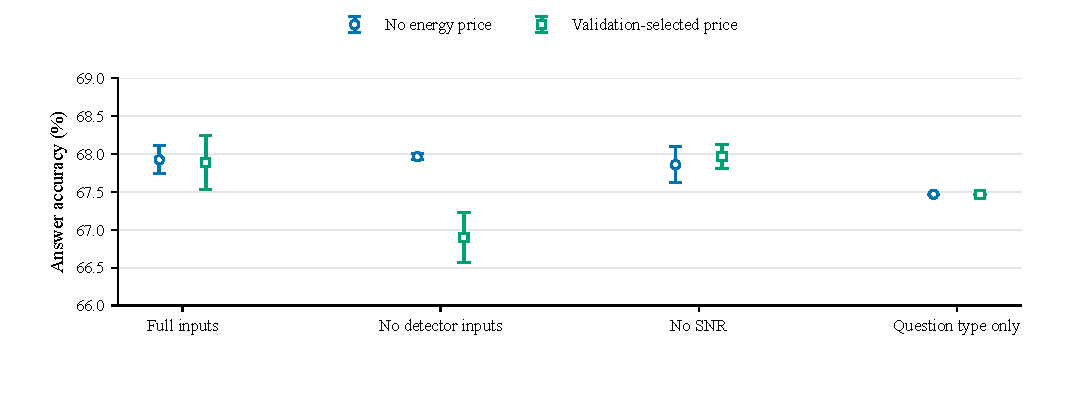
\includegraphics[width=\linewidth]{figures/evidence_final/awgn_ablation.pdf}
\caption{Verified AWGN input ablation. Points show ten-seed mean
accuracy and bars show one sample standard deviation. Both the
zero-price and validation-selected policies are retained.}
\end{figure}

\section{Calibration Control}
VisDrone retains training-only count calibration and an uncalibrated
control. On AWGN, the full MLP's uncalibrated accuracy is
$67.36\%\pm0.18\%$ without an energy price and
$67.22\%\pm0.30\%$ at the validation-selected point.
These are complete re-fits under the corresponding receiver labels,
not post-hoc changes to test answers.

For DroneVehicle, all $24$ class/SNR calibration ratios revert to
$1$ under the training-accuracy acceptance rule. Training, validation,
and test labels are therefore identical in the calibrated and
uncalibrated conditions, as are corresponding seed results.
They are not two independent confirmations of an effect.
The detector remains the VisDrone-trained detector; only the router
is fitted on DroneVehicle training images.

\section{Matched-Receiver Coverage and Adaptation}
Table~\ref{tab:coverage} records the common test workload.
All three receivers use the same keys and received JPEGs, but
coverage differs across question types. Pooling these observations
places more weight on the extra three types than the full VisDrone
test workload.

\begin{table}[t]\centering
\caption{Common matched-receiver test coverage over six SNRs.}
\label{tab:coverage}
\begin{tabular}{@{}lrr@{}}\toprule
Question type & Images & Decisions\\\midrule
Presence & 26 & 624\\
Counting & 26 & 312\\
Comparison & 104 & 624\\
Co-presence & 104 & 624\\
Threshold & 104 & 624\\
\bottomrule\end{tabular}
\end{table}

Restricting test evaluation to the $26$ images with all five types
gives $1{,}404$ decisions. With the same fitted models, mean MLP
accuracies are $67.69\%$, $67.02\%$, and $67.14\%$ for Qwen2-VL,
Qwen2.5-VL, and SmolVLM. These subset values are reported in
addition to, not instead of, the common-key results in the paper.
They show why task composition must accompany an aggregate score.

Receiver-specific MLP image-use fractions are $28.59\%$, $37.59\%$,
and $23.64\%$, respectively. The frozen Qwen2-VL router retains its
$28.59\%$ image-use fraction on both alternative receivers; only
the correctness of the selected target-receiver answer changes.
The SmolVLM transfer loss is therefore not caused by a new target
selection rule. Alternative-receiver energy is not measured,
and these fractions are not converted into empirical energy gains.

\section{Interpretation of Variation and Energy}
The ten seeds quantify training variation on a fixed image split.
They are not ten independent test datasets. Questions, SNRs, and
receiver predictions share images. The present comparisons report
means, sample standard deviations, and descriptive differences;
they do not attach historical bootstrap intervals or equivalence
tests to the revised policies. Any inferential comparison would
need to preserve image clustering and identify its comparison
family. No significance or statistical-equivalence claim is made.

The accounted energy includes modeled transmit and onboard detector
costs and a measured over-idle edge VLM proxy. It excludes image
encoding, router execution, symbolic decoding, flight, sensors,
and radio circuitry. On DroneVehicle, image-only UAV energy is
about $0.132$ J/query, whereas the validation-selected MLP UAV
energy is about $0.450$ J/query. Its lower system energy is
primarily an edge-inference saving. These results must not be
described as a measured UAV battery improvement.
\end{document}
